\documentclass[twoside]{book}

% Packages required by doxygen
\usepackage{fixltx2e}
\usepackage{calc}
\usepackage{doxygen}
\usepackage[export]{adjustbox} % also loads graphicx
\usepackage{graphicx}
\usepackage[utf8]{inputenc}
\usepackage{makeidx}
\usepackage{multicol}
\usepackage{multirow}
\PassOptionsToPackage{warn}{textcomp}
\usepackage{textcomp}
\usepackage[nointegrals]{wasysym}
\usepackage[table]{xcolor}

% Font selection
\usepackage[T1]{fontenc}
\usepackage[scaled=.90]{helvet}
\usepackage{courier}
\usepackage{amssymb}
\usepackage{sectsty}
\renewcommand{\familydefault}{\sfdefault}
\allsectionsfont{%
  \fontseries{bc}\selectfont%
  \color{darkgray}%
}
\renewcommand{\DoxyLabelFont}{%
  \fontseries{bc}\selectfont%
  \color{darkgray}%
}
\newcommand{\+}{\discretionary{\mbox{\scriptsize$\hookleftarrow$}}{}{}}

% Page & text layout
\usepackage{geometry}
\geometry{%
  a4paper,%
  top=2.5cm,%
  bottom=2.5cm,%
  left=2.5cm,%
  right=2.5cm%
}
\tolerance=750
\hfuzz=15pt
\hbadness=750
\setlength{\emergencystretch}{15pt}
\setlength{\parindent}{0cm}
\setlength{\parskip}{3ex plus 2ex minus 2ex}
\makeatletter
\renewcommand{\paragraph}{%
  \@startsection{paragraph}{4}{0ex}{-1.0ex}{1.0ex}{%
    \normalfont\normalsize\bfseries\SS@parafont%
  }%
}
\renewcommand{\subparagraph}{%
  \@startsection{subparagraph}{5}{0ex}{-1.0ex}{1.0ex}{%
    \normalfont\normalsize\bfseries\SS@subparafont%
  }%
}
\makeatother

% Headers & footers
\usepackage{fancyhdr}
\pagestyle{fancyplain}
\fancyhead[LE]{\fancyplain{}{\bfseries\thepage}}
\fancyhead[CE]{\fancyplain{}{}}
\fancyhead[RE]{\fancyplain{}{\bfseries\leftmark}}
\fancyhead[LO]{\fancyplain{}{\bfseries\rightmark}}
\fancyhead[CO]{\fancyplain{}{}}
\fancyhead[RO]{\fancyplain{}{\bfseries\thepage}}
\fancyfoot[LE]{\fancyplain{}{}}
\fancyfoot[CE]{\fancyplain{}{}}
\fancyfoot[RE]{\fancyplain{}{\bfseries\scriptsize Generated by Doxygen }}
\fancyfoot[LO]{\fancyplain{}{\bfseries\scriptsize Generated by Doxygen }}
\fancyfoot[CO]{\fancyplain{}{}}
\fancyfoot[RO]{\fancyplain{}{}}
\renewcommand{\footrulewidth}{0.4pt}
\renewcommand{\chaptermark}[1]{%
  \markboth{#1}{}%
}
\renewcommand{\sectionmark}[1]{%
  \markright{\thesection\ #1}%
}

% Indices & bibliography
\usepackage{natbib}
\usepackage[titles]{tocloft}
\setcounter{tocdepth}{3}
\setcounter{secnumdepth}{5}
\makeindex

% Hyperlinks (required, but should be loaded last)
\usepackage{ifpdf}
\ifpdf
  \usepackage[pdftex,pagebackref=true]{hyperref}
\else
  \usepackage[ps2pdf,pagebackref=true]{hyperref}
\fi
\hypersetup{%
  colorlinks=true,%
  linkcolor=blue,%
  citecolor=blue,%
  unicode%
}

% Custom commands
\newcommand{\clearemptydoublepage}{%
  \newpage{\pagestyle{empty}\cleardoublepage}%
}

\usepackage{caption}
\captionsetup{labelsep=space,justification=centering,font={bf},singlelinecheck=off,skip=4pt,position=top}

%===== C O N T E N T S =====

\begin{document}

% Titlepage & ToC
\hypersetup{pageanchor=false,
             bookmarksnumbered=true,
             pdfencoding=unicode
            }
\pagenumbering{alph}
\begin{titlepage}
\vspace*{7cm}
\begin{center}%
{\Large My Project }\\
\vspace*{1cm}
{\large Generated by Doxygen 1.8.14}\\
\end{center}
\end{titlepage}
\clearemptydoublepage
\pagenumbering{roman}
\tableofcontents
\clearemptydoublepage
\pagenumbering{arabic}
\hypersetup{pageanchor=true}

%--- Begin generated contents ---
\chapter{Hierarchical Index}
\section{Class Hierarchy}
This inheritance list is sorted roughly, but not completely, alphabetically\+:\begin{DoxyCompactList}
\item \contentsline{section}{Edg}{\pageref{class_edg}}{}
\item \contentsline{section}{Edg3}{\pageref{class_edg3}}{}
\item \contentsline{section}{edge}{\pageref{classedge}}{}
\item \contentsline{section}{edge\+\_\+final}{\pageref{classedge__final}}{}
\item \contentsline{section}{main5cpp}{\pageref{classmain5cpp}}{}
\item \contentsline{section}{pair2}{\pageref{classpair2}}{}
\item Q\+Dialog\begin{DoxyCompactList}
\item \contentsline{section}{main\+\_\+choice}{\pageref{classmain__choice}}{}
\end{DoxyCompactList}
\item Q\+G\+L\+Widget\begin{DoxyCompactList}
\item \contentsline{section}{My\+G\+L\+Widget}{\pageref{class_my_g_l_widget}}{}
\end{DoxyCompactList}
\item Q\+Widget\begin{DoxyCompactList}
\item \contentsline{section}{Window}{\pageref{class_window}}{}
\end{DoxyCompactList}
\item \contentsline{section}{Three\+To2\+Main}{\pageref{class_three_to2_main}}{}
\item \contentsline{section}{Ui\+\_\+\+Window}{\pageref{class_ui___window}}{}
\begin{DoxyCompactList}
\item \contentsline{section}{Ui\+:\+:Window}{\pageref{class_ui_1_1_window}}{}
\end{DoxyCompactList}
\item \contentsline{section}{Vert}{\pageref{class_vert}}{}
\item \contentsline{section}{Vert3}{\pageref{class_vert3}}{}
\item \contentsline{section}{vertex}{\pageref{classvertex}}{}
\end{DoxyCompactList}

\chapter{Class Index}
\section{Class List}
Here are the classes, structs, unions and interfaces with brief descriptions\+:\begin{DoxyCompactList}
\item\contentsline{section}{\mbox{\hyperlink{classconstruct3d}{construct3d}} }{\pageref{classconstruct3d}}{}
\item\contentsline{section}{\mbox{\hyperlink{class_edg}{Edg}} }{\pageref{class_edg}}{}
\item\contentsline{section}{\mbox{\hyperlink{class_edg3}{Edg3}} }{\pageref{class_edg3}}{}
\item\contentsline{section}{\mbox{\hyperlink{class_loop}{Loop}} }{\pageref{class_loop}}{}
\item\contentsline{section}{\mbox{\hyperlink{class_vert}{Vert}} }{\pageref{class_vert}}{}
\item\contentsline{section}{\mbox{\hyperlink{class_vert3}{Vert3}} }{\pageref{class_vert3}}{}
\item\contentsline{section}{\mbox{\hyperlink{class_view}{View}} }{\pageref{class_view}}{}
\end{DoxyCompactList}

\chapter{Class Documentation}
\hypertarget{class_edg}{}\section{Edg Class Reference}
\label{class_edg}\index{Edg@{Edg}}
\subsection*{Public Member Functions}
\begin{DoxyCompactItemize}
\item 
\mbox{\Hypertarget{class_edg_a06c3f600f579c9497036558280a13a17}\label{class_edg_a06c3f600f579c9497036558280a13a17}} 
{\bfseries Edg} (\mbox{\hyperlink{class_vert}{Vert}} i1, \mbox{\hyperlink{class_vert}{Vert}} i2)
\end{DoxyCompactItemize}
\subsection*{Public Attributes}
\begin{DoxyCompactItemize}
\item 
\mbox{\Hypertarget{class_edg_a1bf2dfdbef7d62f34c9cd08469154491}\label{class_edg_a1bf2dfdbef7d62f34c9cd08469154491}} 
\mbox{\hyperlink{class_vert}{Vert}} {\bfseries s}
\item 
\mbox{\Hypertarget{class_edg_ab3fb9fd99e35eabeba6eed911cbb7f93}\label{class_edg_ab3fb9fd99e35eabeba6eed911cbb7f93}} 
\mbox{\hyperlink{class_vert}{Vert}} {\bfseries e}
\end{DoxyCompactItemize}


The documentation for this class was generated from the following file\+:\begin{DoxyCompactItemize}
\item 
main5cpp.\+h\end{DoxyCompactItemize}

\hypertarget{class_edg3}{}\section{Edg3 Class Reference}
\label{class_edg3}\index{Edg3@{Edg3}}
\subsection*{Public Member Functions}
\begin{DoxyCompactItemize}
\item 
\mbox{\Hypertarget{class_edg3_a97ef4425690e064ad10ed13e179a2874}\label{class_edg3_a97ef4425690e064ad10ed13e179a2874}} 
{\bfseries Edg3} (\mbox{\hyperlink{class_vert3}{Vert3}} v1, \mbox{\hyperlink{class_vert3}{Vert3}} v2)
\end{DoxyCompactItemize}
\subsection*{Public Attributes}
\begin{DoxyCompactItemize}
\item 
\mbox{\Hypertarget{class_edg3_a1f391c8ccb863a19bd143d31493db77a}\label{class_edg3_a1f391c8ccb863a19bd143d31493db77a}} 
\mbox{\hyperlink{class_vert3}{Vert3}} {\bfseries s}
\item 
\mbox{\Hypertarget{class_edg3_a090172b8938032a52b12875768395faa}\label{class_edg3_a090172b8938032a52b12875768395faa}} 
\mbox{\hyperlink{class_vert3}{Vert3}} {\bfseries e}
\end{DoxyCompactItemize}


The documentation for this class was generated from the following file\+:\begin{DoxyCompactItemize}
\item 
main5cpp.\+h\end{DoxyCompactItemize}

\hypertarget{classedge}{}\section{edge Class Reference}
\label{classedge}\index{edge@{edge}}
\subsection*{Public Member Functions}
\begin{DoxyCompactItemize}
\item 
\mbox{\Hypertarget{classedge_a810a8bbcaa60304c654bd6bbfe1915b0}\label{classedge_a810a8bbcaa60304c654bd6bbfe1915b0}} 
{\bfseries edge} (int e1, int e2, bool b)
\item 
\mbox{\Hypertarget{classedge_af6c75391caaee88d8ffb2331641eb531}\label{classedge_af6c75391caaee88d8ffb2331641eb531}} 
bool {\bfseries operator==} (const \mbox{\hyperlink{classedge}{edge}} \&rhs) const
\end{DoxyCompactItemize}
\subsection*{Public Attributes}
\begin{DoxyCompactItemize}
\item 
\mbox{\Hypertarget{classedge_a08a065565db6999f12fd4498422e115c}\label{classedge_a08a065565db6999f12fd4498422e115c}} 
int {\bfseries x}
\item 
\mbox{\Hypertarget{classedge_a24d6d9ad1d9309c0ce3b40c3dcd6b623}\label{classedge_a24d6d9ad1d9309c0ce3b40c3dcd6b623}} 
int {\bfseries y}
\item 
\mbox{\Hypertarget{classedge_a58e9f0be7697205f09966afeb70bd459}\label{classedge_a58e9f0be7697205f09966afeb70bd459}} 
bool {\bfseries hidden}
\end{DoxyCompactItemize}


The documentation for this class was generated from the following files\+:\begin{DoxyCompactItemize}
\item 
classes.\+h\item 
classes.\+cpp\end{DoxyCompactItemize}

\hypertarget{classedge__final}{}\section{edge\+\_\+final Class Reference}
\label{classedge__final}\index{edge\+\_\+final@{edge\+\_\+final}}
\subsection*{Public Member Functions}
\begin{DoxyCompactItemize}
\item 
\mbox{\Hypertarget{classedge__final_a4225d843dc9446daea26c9d132c4a52e}\label{classedge__final_a4225d843dc9446daea26c9d132c4a52e}} 
{\bfseries edge\+\_\+final} (\mbox{\hyperlink{classpair2}{pair2}} source, \mbox{\hyperlink{classpair2}{pair2}} destination, bool h)
\end{DoxyCompactItemize}
\subsection*{Public Attributes}
\begin{DoxyCompactItemize}
\item 
\mbox{\Hypertarget{classedge__final_ae6182a6d67ff0c962963349e23a2f73c}\label{classedge__final_ae6182a6d67ff0c962963349e23a2f73c}} 
\mbox{\hyperlink{classpair2}{pair2}} {\bfseries p1}
\item 
\mbox{\Hypertarget{classedge__final_a44f33f94dd704714fc5ddf9cd47dc5b4}\label{classedge__final_a44f33f94dd704714fc5ddf9cd47dc5b4}} 
\mbox{\hyperlink{classpair2}{pair2}} {\bfseries p2}
\item 
\mbox{\Hypertarget{classedge__final_af6e0c638afa6d69c69ec7f9c3df041cf}\label{classedge__final_af6e0c638afa6d69c69ec7f9c3df041cf}} 
bool {\bfseries hidden}
\end{DoxyCompactItemize}


The documentation for this class was generated from the following files\+:\begin{DoxyCompactItemize}
\item 
classes.\+h\item 
classes.\+cpp\end{DoxyCompactItemize}

\hypertarget{classmain5cpp}{}\section{main5cpp Class Reference}
\label{classmain5cpp}\index{main5cpp@{main5cpp}}


The documentation for this class was generated from the following file\+:\begin{DoxyCompactItemize}
\item 
main5cpp.\+h\end{DoxyCompactItemize}

\hypertarget{classmain__choice}{}\section{main\+\_\+choice Class Reference}
\label{classmain__choice}\index{main\+\_\+choice@{main\+\_\+choice}}
Inheritance diagram for main\+\_\+choice\+:\begin{figure}[H]
\begin{center}
\leavevmode
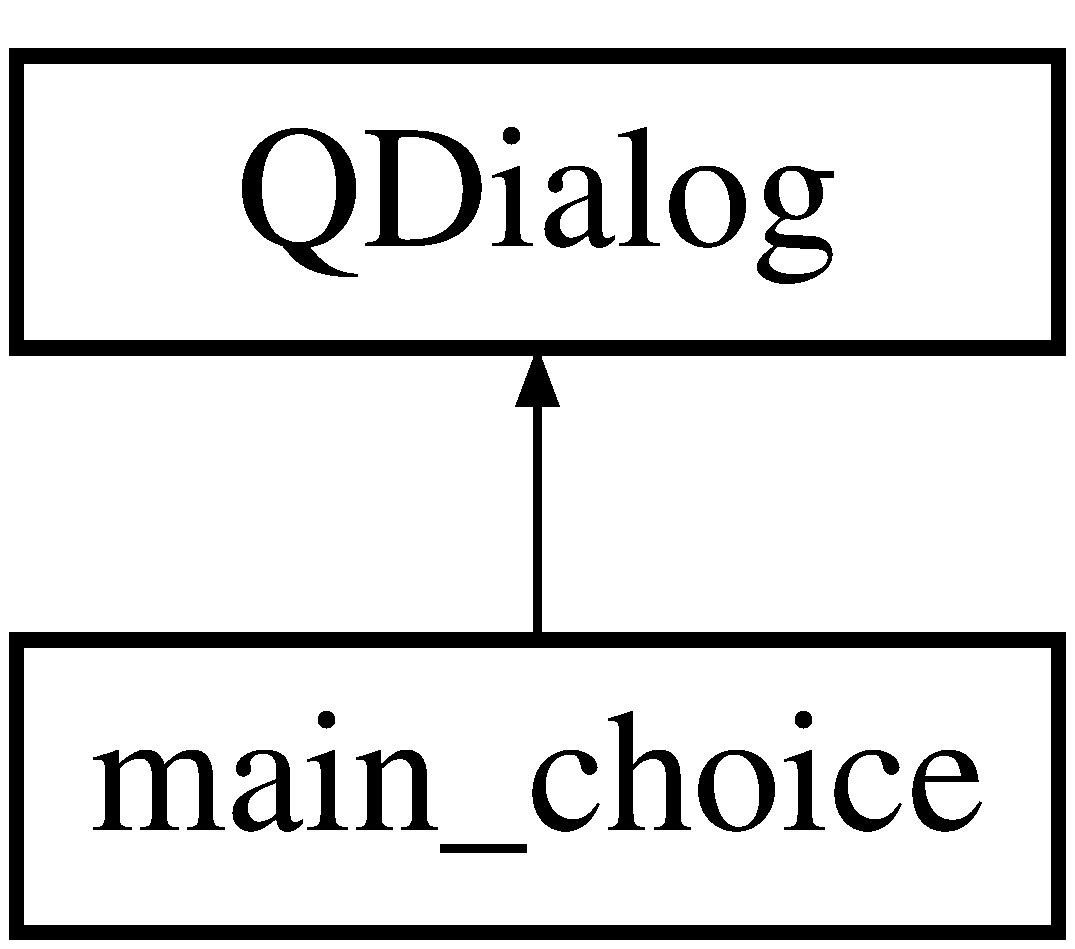
\includegraphics[height=2.000000cm]{classmain__choice}
\end{center}
\end{figure}
\subsection*{Public Slots}
\begin{DoxyCompactItemize}
\item 
\mbox{\Hypertarget{classmain__choice_a2982ce0c586042302c93288214b87a94}\label{classmain__choice_a2982ce0c586042302c93288214b87a94}} 
void {\bfseries on\+\_\+\+Two\+D\+\_\+to\+\_\+3\+D\+\_\+clicked} ()
\item 
\mbox{\Hypertarget{classmain__choice_aba751377bcb77dd148b20dcac4e7137c}\label{classmain__choice_aba751377bcb77dd148b20dcac4e7137c}} 
void {\bfseries on\+\_\+\+Three\+D\+\_\+to\+\_\+2\+D\+\_\+o\+\_\+clicked} ()
\item 
\mbox{\Hypertarget{classmain__choice_af3e5bf8f7a7524cc57635063ed629b2b}\label{classmain__choice_af3e5bf8f7a7524cc57635063ed629b2b}} 
void {\bfseries on\+\_\+\+Three\+D\+\_\+to\+\_\+2\+D\+\_\+dr\+\_\+clicked} ()
\end{DoxyCompactItemize}
\subsection*{Public Member Functions}
\begin{DoxyCompactItemize}
\item 
\mbox{\Hypertarget{classmain__choice_af3597c64880a8aab73fe55f125ffc995}\label{classmain__choice_af3597c64880a8aab73fe55f125ffc995}} 
{\bfseries main\+\_\+choice} (Q\+Widget $\ast$parent=0)
\end{DoxyCompactItemize}


The documentation for this class was generated from the following files\+:\begin{DoxyCompactItemize}
\item 
main\+\_\+choice.\+h\item 
main.\+cpp\end{DoxyCompactItemize}

\hypertarget{class_my_g_l_widget}{}\section{My\+G\+L\+Widget Class Reference}
\label{class_my_g_l_widget}\index{My\+G\+L\+Widget@{My\+G\+L\+Widget}}
Inheritance diagram for My\+G\+L\+Widget\+:\begin{figure}[H]
\begin{center}
\leavevmode
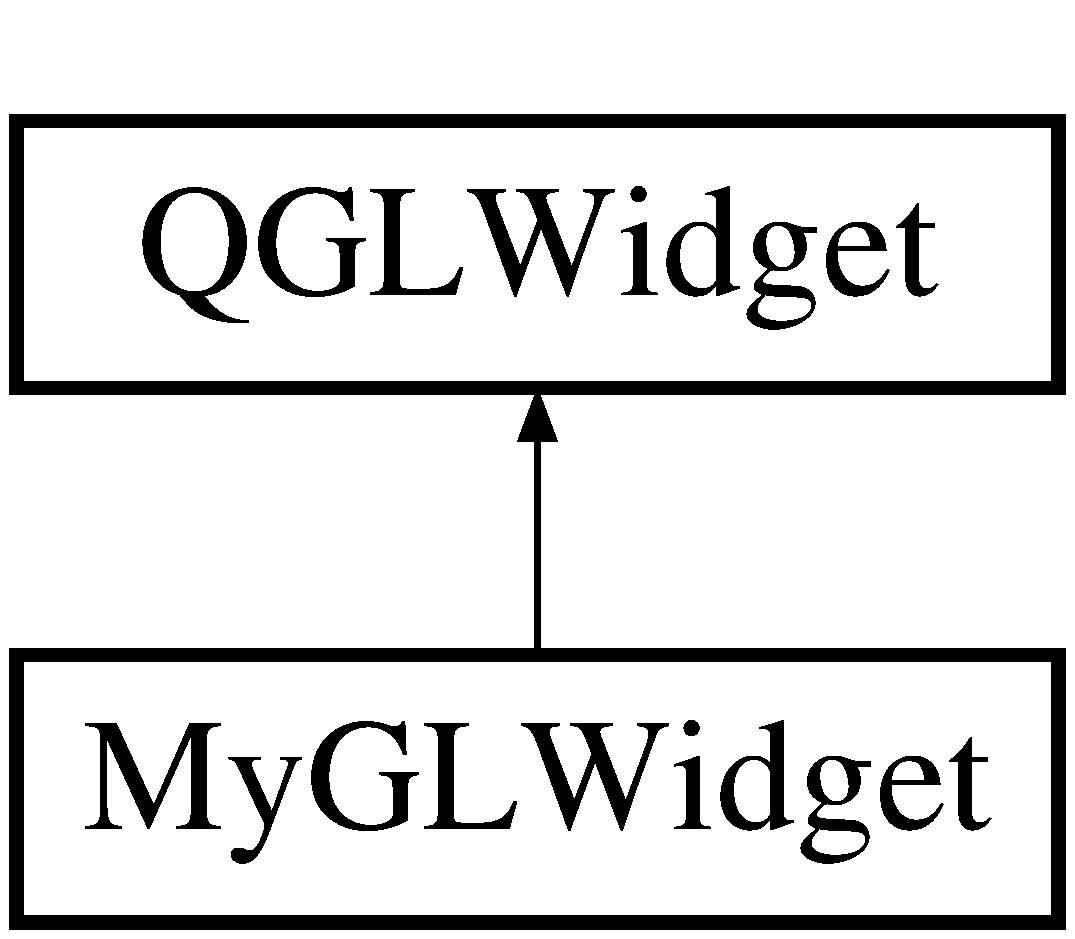
\includegraphics[height=2.000000cm]{class_my_g_l_widget}
\end{center}
\end{figure}
\subsection*{Public Slots}
\begin{DoxyCompactItemize}
\item 
\mbox{\Hypertarget{class_my_g_l_widget_ae25d0d92cce067011b007d2981a73cf5}\label{class_my_g_l_widget_ae25d0d92cce067011b007d2981a73cf5}} 
void {\bfseries set\+X\+Rotation} (int angle)
\item 
\mbox{\Hypertarget{class_my_g_l_widget_abcd9fa6194011d563c281b723fdf5212}\label{class_my_g_l_widget_abcd9fa6194011d563c281b723fdf5212}} 
void {\bfseries set\+Y\+Rotation} (int angle)
\item 
\mbox{\Hypertarget{class_my_g_l_widget_aa54d51fa4a18e3fba20ceaa643bb2bea}\label{class_my_g_l_widget_aa54d51fa4a18e3fba20ceaa643bb2bea}} 
void {\bfseries set\+Z\+Rotation} (int angle)
\end{DoxyCompactItemize}
\subsection*{Signals}
\begin{DoxyCompactItemize}
\item 
\mbox{\Hypertarget{class_my_g_l_widget_a4b68ba3a94f33acd2a7c6378b6e0d8c4}\label{class_my_g_l_widget_a4b68ba3a94f33acd2a7c6378b6e0d8c4}} 
void {\bfseries x\+Rotation\+Changed} (int angle)
\item 
\mbox{\Hypertarget{class_my_g_l_widget_a6b8d69c457500f1d991b95f5e56c69c3}\label{class_my_g_l_widget_a6b8d69c457500f1d991b95f5e56c69c3}} 
void {\bfseries y\+Rotation\+Changed} (int angle)
\item 
\mbox{\Hypertarget{class_my_g_l_widget_a29cd77996caf2a33c4d82c1b2a923689}\label{class_my_g_l_widget_a29cd77996caf2a33c4d82c1b2a923689}} 
void {\bfseries z\+Rotation\+Changed} (int angle)
\end{DoxyCompactItemize}
\subsection*{Public Member Functions}
\begin{DoxyCompactItemize}
\item 
\mbox{\Hypertarget{class_my_g_l_widget_a2b3f2523eae378b2a4a5f66bd176be57}\label{class_my_g_l_widget_a2b3f2523eae378b2a4a5f66bd176be57}} 
{\bfseries My\+G\+L\+Widget} (Q\+Widget $\ast$parent=0)
\end{DoxyCompactItemize}
\subsection*{Protected Member Functions}
\begin{DoxyCompactItemize}
\item 
\mbox{\Hypertarget{class_my_g_l_widget_a5c536c2ebab76533eb16eac0a9830c8e}\label{class_my_g_l_widget_a5c536c2ebab76533eb16eac0a9830c8e}} 
void {\bfseries initialize\+GL} ()
\item 
\mbox{\Hypertarget{class_my_g_l_widget_ad0e4171fab09ad54d4e2d23e7d6541eb}\label{class_my_g_l_widget_ad0e4171fab09ad54d4e2d23e7d6541eb}} 
void {\bfseries paint\+GL} ()
\item 
\mbox{\Hypertarget{class_my_g_l_widget_a9717968e75b8a7fc358b947f31eb2690}\label{class_my_g_l_widget_a9717968e75b8a7fc358b947f31eb2690}} 
void {\bfseries resize\+GL} (int width, int height)
\item 
\mbox{\Hypertarget{class_my_g_l_widget_af0c7693331391d76bb55c8de43045432}\label{class_my_g_l_widget_af0c7693331391d76bb55c8de43045432}} 
Q\+Size {\bfseries minimum\+Size\+Hint} () const
\item 
\mbox{\Hypertarget{class_my_g_l_widget_a38801d23bead00f1345eb62566155782}\label{class_my_g_l_widget_a38801d23bead00f1345eb62566155782}} 
Q\+Size {\bfseries size\+Hint} () const
\item 
\mbox{\Hypertarget{class_my_g_l_widget_a2bcae28bda70b99245164f55b847679a}\label{class_my_g_l_widget_a2bcae28bda70b99245164f55b847679a}} 
void {\bfseries mouse\+Press\+Event} (Q\+Mouse\+Event $\ast$event)
\item 
\mbox{\Hypertarget{class_my_g_l_widget_a519efceb466527b8730d82ee1a0da8fb}\label{class_my_g_l_widget_a519efceb466527b8730d82ee1a0da8fb}} 
void {\bfseries mouse\+Move\+Event} (Q\+Mouse\+Event $\ast$event)
\end{DoxyCompactItemize}


The documentation for this class was generated from the following files\+:\begin{DoxyCompactItemize}
\item 
myglwidget.\+h\item 
myglwidget.\+cpp\end{DoxyCompactItemize}

\hypertarget{classpair2}{}\section{pair2 Class Reference}
\label{classpair2}\index{pair2@{pair2}}
\subsection*{Public Member Functions}
\begin{DoxyCompactItemize}
\item 
\mbox{\Hypertarget{classpair2_adb1a9362760bb925295f3422f1df424b}\label{classpair2_adb1a9362760bb925295f3422f1df424b}} 
{\bfseries pair2} (double i1, double i2)
\item 
\mbox{\Hypertarget{classpair2_ad28c08f071dfb7ddae18e4d5ea9ea9c1}\label{classpair2_ad28c08f071dfb7ddae18e4d5ea9ea9c1}} 
bool {\bfseries operator$<$} (const \mbox{\hyperlink{classpair2}{pair2}} \&src) const
\item 
\mbox{\Hypertarget{classpair2_abf5a0ceb5035f744f6dabdf6a97902bf}\label{classpair2_abf5a0ceb5035f744f6dabdf6a97902bf}} 
bool {\bfseries operator==} (const \mbox{\hyperlink{classpair2}{pair2}} \&rhs) const
\item 
\mbox{\Hypertarget{classpair2_a7c6b5eaef6f52bc68ea3ed3437752769}\label{classpair2_a7c6b5eaef6f52bc68ea3ed3437752769}} 
bool {\bfseries intersect} (\mbox{\hyperlink{classpair2}{pair2}} p1, \mbox{\hyperlink{classpair2}{pair2}} p2)
\end{DoxyCompactItemize}
\subsection*{Public Attributes}
\begin{DoxyCompactItemize}
\item 
\mbox{\Hypertarget{classpair2_a3642c27aff74f421549132c0f8b806da}\label{classpair2_a3642c27aff74f421549132c0f8b806da}} 
double {\bfseries x}
\item 
\mbox{\Hypertarget{classpair2_a97b0eb83e4dcb38ad24f3c26e0c2fed7}\label{classpair2_a97b0eb83e4dcb38ad24f3c26e0c2fed7}} 
double {\bfseries y}
\end{DoxyCompactItemize}


The documentation for this class was generated from the following files\+:\begin{DoxyCompactItemize}
\item 
classes.\+h\item 
classes.\+cpp\end{DoxyCompactItemize}

\hypertarget{class_three_to2_main}{}\section{Three\+To2\+Main Class Reference}
\label{class_three_to2_main}\index{Three\+To2\+Main@{Three\+To2\+Main}}


The documentation for this class was generated from the following files\+:\begin{DoxyCompactItemize}
\item 
threeto2main.\+h\item 
main.\+cpp\end{DoxyCompactItemize}

\hypertarget{class_ui___window}{}\section{Ui\+\_\+\+Window Class Reference}
\label{class_ui___window}\index{Ui\+\_\+\+Window@{Ui\+\_\+\+Window}}
Inheritance diagram for Ui\+\_\+\+Window\+:\begin{figure}[H]
\begin{center}
\leavevmode
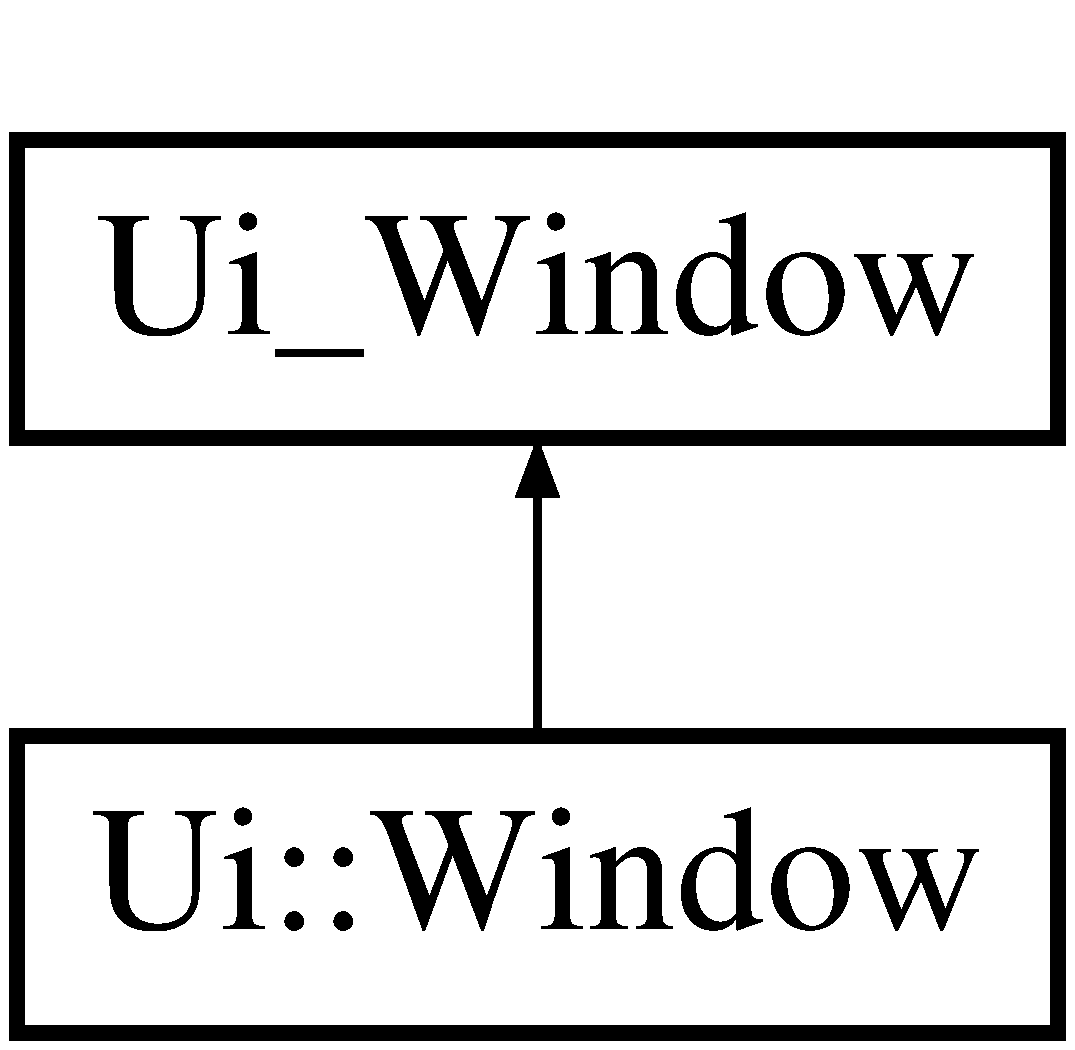
\includegraphics[height=2.000000cm]{class_ui___window}
\end{center}
\end{figure}
\subsection*{Public Member Functions}
\begin{DoxyCompactItemize}
\item 
\mbox{\Hypertarget{class_ui___window_adaef25b7c1b0e3791a28344412c7c3ee}\label{class_ui___window_adaef25b7c1b0e3791a28344412c7c3ee}} 
void {\bfseries setup\+Ui} (Q\+Widget $\ast$\mbox{\hyperlink{class_window}{Window}})
\item 
\mbox{\Hypertarget{class_ui___window_ad3eaf2336ed8418baad54d6703daaeea}\label{class_ui___window_ad3eaf2336ed8418baad54d6703daaeea}} 
void {\bfseries retranslate\+Ui} (Q\+Widget $\ast$\mbox{\hyperlink{class_window}{Window}})
\end{DoxyCompactItemize}
\subsection*{Public Attributes}
\begin{DoxyCompactItemize}
\item 
\mbox{\Hypertarget{class_ui___window_afb9bb0a79fe82f343bcfd69794590ae8}\label{class_ui___window_afb9bb0a79fe82f343bcfd69794590ae8}} 
Q\+V\+Box\+Layout $\ast$ {\bfseries vertical\+Layout}
\item 
\mbox{\Hypertarget{class_ui___window_afdc55bf84d9d31159c56d7b1220077d0}\label{class_ui___window_afdc55bf84d9d31159c56d7b1220077d0}} 
\mbox{\hyperlink{class_my_g_l_widget}{My\+G\+L\+Widget}} $\ast$ {\bfseries my\+G\+L\+Widget}
\item 
\mbox{\Hypertarget{class_ui___window_a167433b4f13baf636c5449a47327c957}\label{class_ui___window_a167433b4f13baf636c5449a47327c957}} 
Q\+H\+Box\+Layout $\ast$ {\bfseries horizontal\+Layout}
\item 
\mbox{\Hypertarget{class_ui___window_af91af662a3516cccfdfddb0ac0c6c32c}\label{class_ui___window_af91af662a3516cccfdfddb0ac0c6c32c}} 
Q\+Label $\ast$ {\bfseries label}
\item 
\mbox{\Hypertarget{class_ui___window_a8b0d45d82bee3eec8c9e44e88fd7bb94}\label{class_ui___window_a8b0d45d82bee3eec8c9e44e88fd7bb94}} 
Q\+Slider $\ast$ {\bfseries rot\+X\+Slider}
\item 
\mbox{\Hypertarget{class_ui___window_a2d5fbd674cd5e137b9f482a12762ac48}\label{class_ui___window_a2d5fbd674cd5e137b9f482a12762ac48}} 
Q\+H\+Box\+Layout $\ast$ {\bfseries horizontal\+Layout\+\_\+2}
\item 
\mbox{\Hypertarget{class_ui___window_aab7d650781ef514a9abb6a83fb44317e}\label{class_ui___window_aab7d650781ef514a9abb6a83fb44317e}} 
Q\+Label $\ast$ {\bfseries label\+\_\+2}
\item 
\mbox{\Hypertarget{class_ui___window_a67120fe99326079b0f332ef837289915}\label{class_ui___window_a67120fe99326079b0f332ef837289915}} 
Q\+Slider $\ast$ {\bfseries rot\+Y\+Slider}
\item 
\mbox{\Hypertarget{class_ui___window_ace5df3a15fbcf6208783b7198e7d9a42}\label{class_ui___window_ace5df3a15fbcf6208783b7198e7d9a42}} 
Q\+H\+Box\+Layout $\ast$ {\bfseries horizontal\+Layout\+\_\+3}
\item 
\mbox{\Hypertarget{class_ui___window_a42fbf07a01626d3d90c0606592d5ff91}\label{class_ui___window_a42fbf07a01626d3d90c0606592d5ff91}} 
Q\+Label $\ast$ {\bfseries label\+\_\+3}
\item 
\mbox{\Hypertarget{class_ui___window_a7a412845d75ad8b4f85959a6afba9685}\label{class_ui___window_a7a412845d75ad8b4f85959a6afba9685}} 
Q\+Slider $\ast$ {\bfseries rot\+Z\+Slider}
\end{DoxyCompactItemize}


The documentation for this class was generated from the following file\+:\begin{DoxyCompactItemize}
\item 
ui\+\_\+window.\+h\end{DoxyCompactItemize}

\hypertarget{class_vert}{}\section{Vert Class Reference}
\label{class_vert}\index{Vert@{Vert}}
\subsection*{Public Member Functions}
\begin{DoxyCompactItemize}
\item 
\mbox{\Hypertarget{class_vert_adafd82053d5532a81753ffca27465d98}\label{class_vert_adafd82053d5532a81753ffca27465d98}} 
{\bfseries Vert} (double i1, double i2)
\item 
\mbox{\Hypertarget{class_vert_ab1144e4319c8a143468d11bb3dd45347}\label{class_vert_ab1144e4319c8a143468d11bb3dd45347}} 
bool {\bfseries operator==} (const \mbox{\hyperlink{class_vert}{Vert}} \&rhs)
\end{DoxyCompactItemize}
\subsection*{Public Attributes}
\begin{DoxyCompactItemize}
\item 
\mbox{\Hypertarget{class_vert_a4a7108e232ab803e8977b37ac4efaf99}\label{class_vert_a4a7108e232ab803e8977b37ac4efaf99}} 
double {\bfseries c1}
\item 
\mbox{\Hypertarget{class_vert_a9bc58ca1af5fc074fcc303c2432d64b0}\label{class_vert_a9bc58ca1af5fc074fcc303c2432d64b0}} 
double {\bfseries c2}
\end{DoxyCompactItemize}


The documentation for this class was generated from the following file\+:\begin{DoxyCompactItemize}
\item 
main5cpp.\+h\end{DoxyCompactItemize}

\hypertarget{class_vert3}{}\section{Vert3 Class Reference}
\label{class_vert3}\index{Vert3@{Vert3}}
\subsection*{Public Member Functions}
\begin{DoxyCompactItemize}
\item 
\mbox{\Hypertarget{class_vert3_a09911f7edcf7f87c2bd730e6638cc0a6}\label{class_vert3_a09911f7edcf7f87c2bd730e6638cc0a6}} 
{\bfseries Vert3} (\mbox{\hyperlink{class_vert}{Vert}} v1, \mbox{\hyperlink{class_vert}{Vert}} v2)
\end{DoxyCompactItemize}
\subsection*{Public Attributes}
\begin{DoxyCompactItemize}
\item 
\mbox{\Hypertarget{class_vert3_a1b2cd0d7f85932f58fad5765e03fa32e}\label{class_vert3_a1b2cd0d7f85932f58fad5765e03fa32e}} 
double {\bfseries x}
\item 
\mbox{\Hypertarget{class_vert3_adcf98f8e6a291e0895fa81a17b9ae2f0}\label{class_vert3_adcf98f8e6a291e0895fa81a17b9ae2f0}} 
double {\bfseries y}
\item 
\mbox{\Hypertarget{class_vert3_a51bc9dcad09b7ed8736f468910ef25fd}\label{class_vert3_a51bc9dcad09b7ed8736f468910ef25fd}} 
double {\bfseries z}
\end{DoxyCompactItemize}


The documentation for this class was generated from the following file\+:\begin{DoxyCompactItemize}
\item 
main5cpp.\+h\end{DoxyCompactItemize}

\hypertarget{classvertex}{}\section{vertex Class Reference}
\label{classvertex}\index{vertex@{vertex}}
\subsection*{Public Member Functions}
\begin{DoxyCompactItemize}
\item 
\mbox{\Hypertarget{classvertex_a90609a1a7ca0891ece57daa80d7601b3}\label{classvertex_a90609a1a7ca0891ece57daa80d7601b3}} 
{\bfseries vertex} (double i1, double i2, double i3)
\end{DoxyCompactItemize}
\subsection*{Public Attributes}
\begin{DoxyCompactItemize}
\item 
\mbox{\Hypertarget{classvertex_a11f52ec2e920d56500baefe5a2e2bba7}\label{classvertex_a11f52ec2e920d56500baefe5a2e2bba7}} 
double {\bfseries x}
\item 
\mbox{\Hypertarget{classvertex_a8b9f211498390a67c369fd43f3722a19}\label{classvertex_a8b9f211498390a67c369fd43f3722a19}} 
double {\bfseries y}
\item 
\mbox{\Hypertarget{classvertex_a4e4f9696a91e9bee75a4c15d8d77e064}\label{classvertex_a4e4f9696a91e9bee75a4c15d8d77e064}} 
double {\bfseries z}
\end{DoxyCompactItemize}


The documentation for this class was generated from the following files\+:\begin{DoxyCompactItemize}
\item 
classes.\+h\item 
classes.\+cpp\end{DoxyCompactItemize}

\hypertarget{class_ui_1_1_window}{}\section{Ui\+:\+:Window Class Reference}
\label{class_ui_1_1_window}\index{Ui\+::\+Window@{Ui\+::\+Window}}
Inheritance diagram for Ui\+:\+:Window\+:\begin{figure}[H]
\begin{center}
\leavevmode
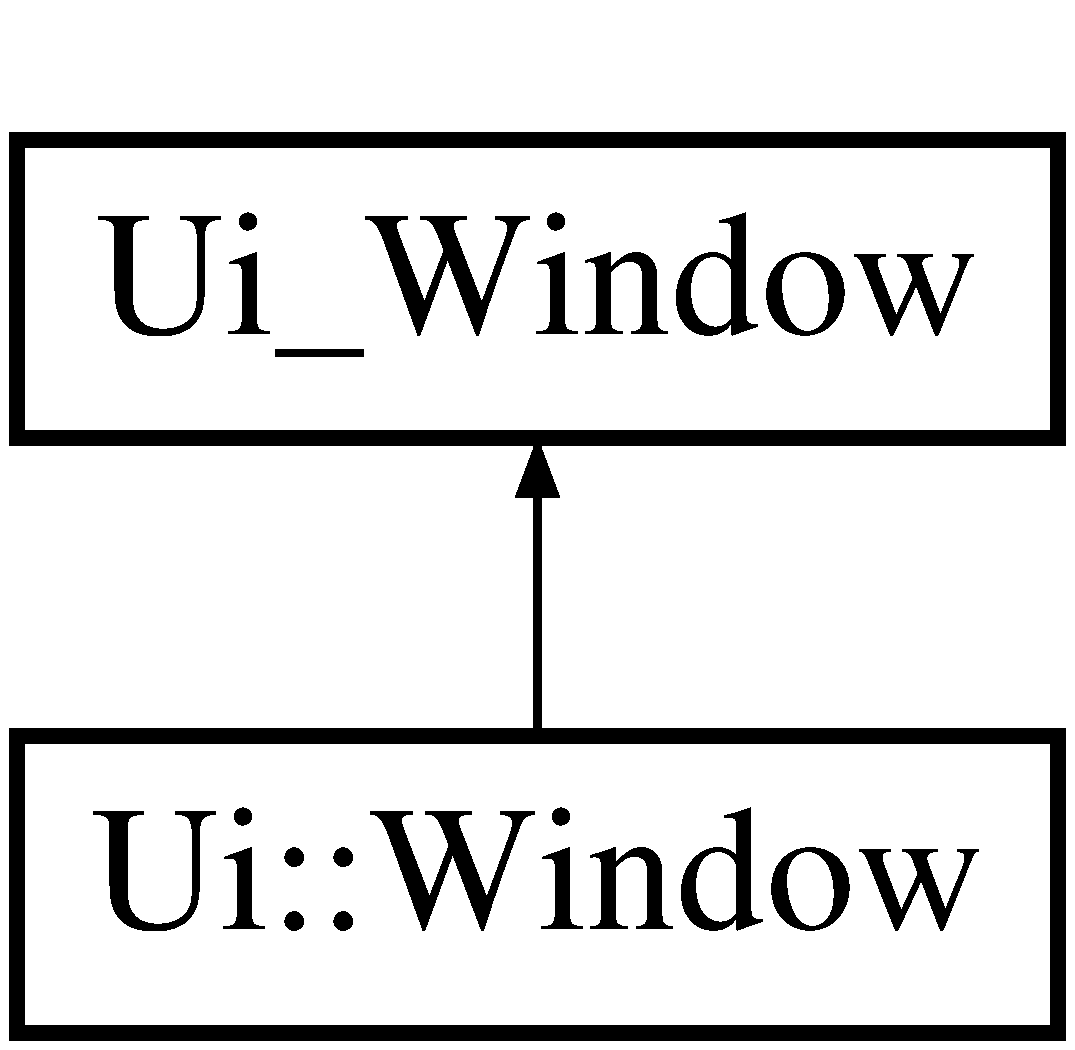
\includegraphics[height=2.000000cm]{class_ui_1_1_window}
\end{center}
\end{figure}
\subsection*{Additional Inherited Members}


The documentation for this class was generated from the following file\+:\begin{DoxyCompactItemize}
\item 
ui\+\_\+window.\+h\end{DoxyCompactItemize}

\hypertarget{class_window}{}\section{Window Class Reference}
\label{class_window}\index{Window@{Window}}
Inheritance diagram for Window\+:\begin{figure}[H]
\begin{center}
\leavevmode
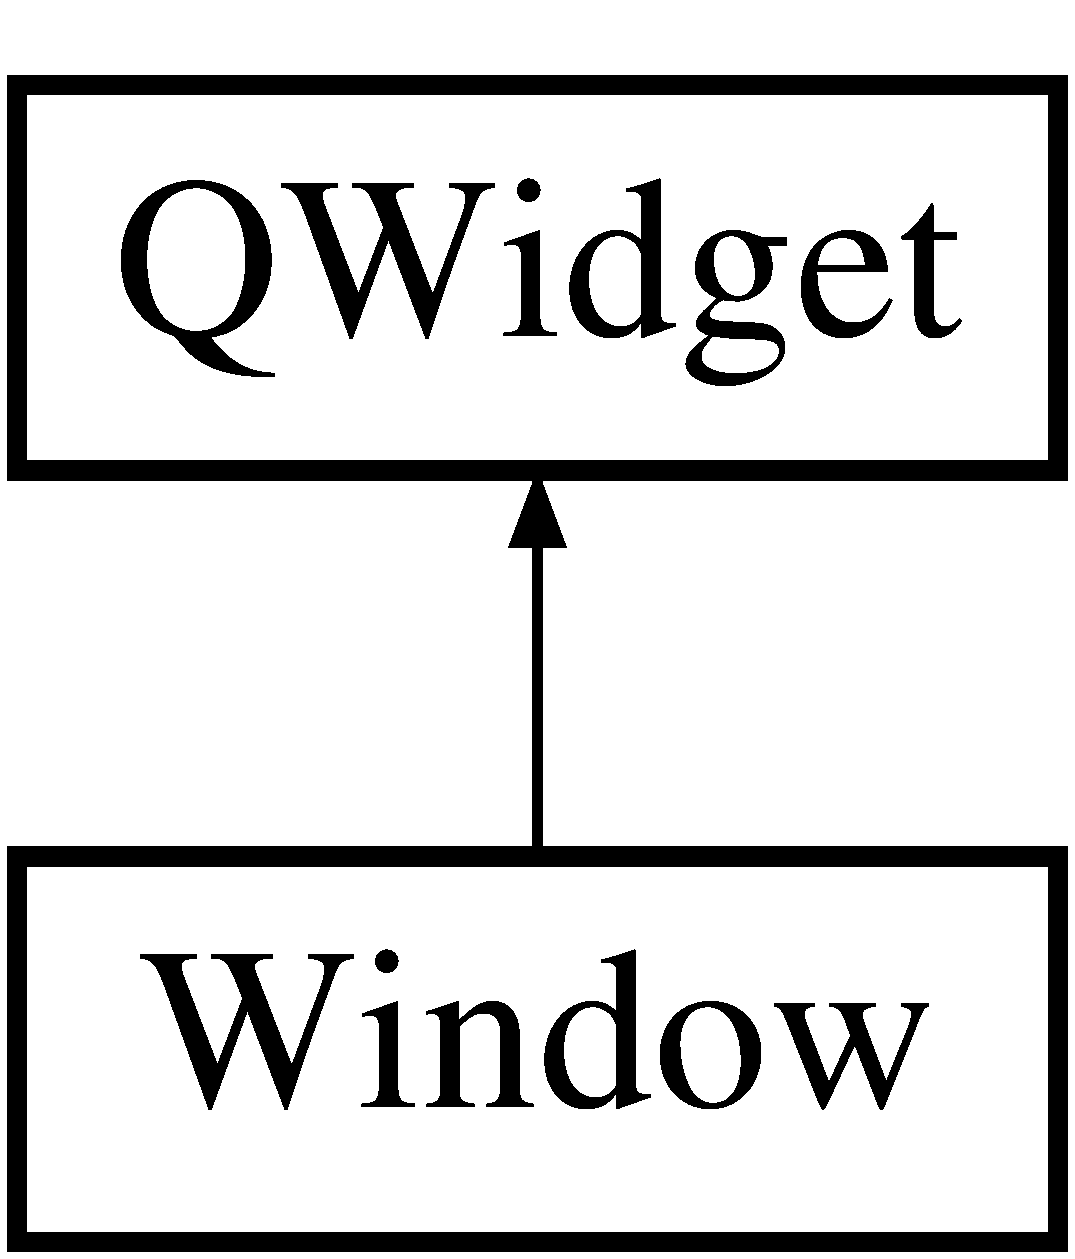
\includegraphics[height=2.000000cm]{class_window}
\end{center}
\end{figure}
\subsection*{Public Member Functions}
\begin{DoxyCompactItemize}
\item 
\mbox{\Hypertarget{class_window_ab27fe44e0834066236f79f244b02f67e}\label{class_window_ab27fe44e0834066236f79f244b02f67e}} 
{\bfseries Window} (Q\+Widget $\ast$parent=0)
\end{DoxyCompactItemize}
\subsection*{Protected Member Functions}
\begin{DoxyCompactItemize}
\item 
\mbox{\Hypertarget{class_window_a52322a90bc51afcd17b90a152d64f36a}\label{class_window_a52322a90bc51afcd17b90a152d64f36a}} 
void {\bfseries key\+Press\+Event} (Q\+Key\+Event $\ast$event)
\end{DoxyCompactItemize}


The documentation for this class was generated from the following files\+:\begin{DoxyCompactItemize}
\item 
window.\+h\item 
window.\+cpp\end{DoxyCompactItemize}

%--- End generated contents ---

% Index
\backmatter
\newpage
\phantomsection
\clearemptydoublepage
\addcontentsline{toc}{chapter}{Index}
\printindex

\end{document}
